%
% fig/bisektion.tex -- Bisektion auf R
%
\begin{figure}
\centering
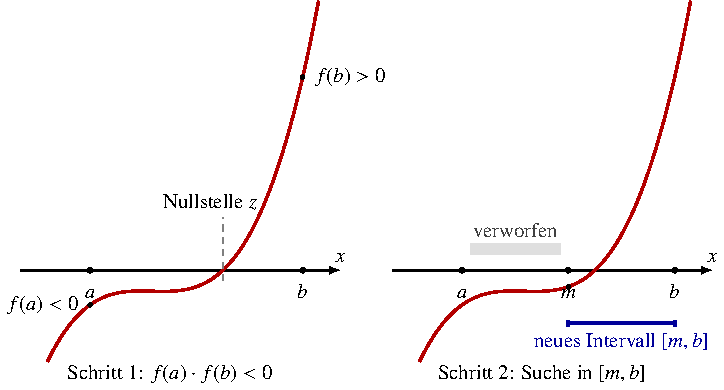
\includegraphics{papers/weyl/images/bisektion.pdf}
\caption{Bisektion einer reellen stetigen Funktion: das Vorzeichen wechselt
zwischen $a$ und $b$, also liegt nach dem Zwischenwertsatz mindestens eine
Nullstelle dazwischen. Durch Halbieren und Auswählen der Hälfte mit
Vorzeichenwechsel verkleinert sich der Suchbereich pro Schritt um den Faktor zwei.
\label{weyl:fig:bisektion}}
\end{figure}
